\section{Motivating example}
In this section, we formulate the problem of context-free path query evaluation on a small graph with classical \textit{same-generation query}~\cite{FndDB} which cannot be expressed by regular expressions.

Suppose that we have a graph database or any other object which has a graph representation. The same-generation query is useful for discovering vertex similarity in this representation. For example, this kind of queries can be applied to gene similarity discovery~\cite{GraphQueryWithEarley}. For graph databases, the same-generation query evaluation consists on finding all the nodes at the same level of a hierarchy. The language formed by paths between such nodes is not regular and corresponds to the language of strings containing matching parentheses. Hence, this query formulated as a context-free grammar.

For this example, we have a small double-cyclic graph, shown in Figure~\ref{Example_Graph}. One of the cycles having three edges labeled with $a$, and one having two edges labeled with $b$. The two cycles are connected via
a shared node $0$.

\begin{figure}[h]
	\[
	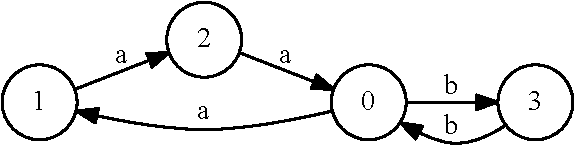
\includegraphics[width=7cm]{pictures/example_graph.pdf}
	\]
	\caption{An example graph.}
	\label{Example_Graph}
\end{figure}

For this graph, we have a same-generation query formulated as a context-free grammar which generates a context-free language $L=\{a^n b^n; n \geq 1\}$.

The result of context-free path query evaluation on this example is a set of node pairs $(m, n)$, such that there is a path from the node $m$ to the node $n$, whose labeling form a string from the language $L$. For example, the node pair $(0,0)$ must be in this set, since there is a path from the node $0$ to the node $0$, whose labeling form a string $w = aaaaaabbbbbb = a^6b^6 \in L$.

Further, in this paper, we show how this problem can be solved with active using of matrix operations.